\newpage
\section*{Appendix}
\label{app:appendix}

\subsection*{AlexNet Model}
\label{app:appendix_alexnet_model}
\begin{figure}
    \centering
    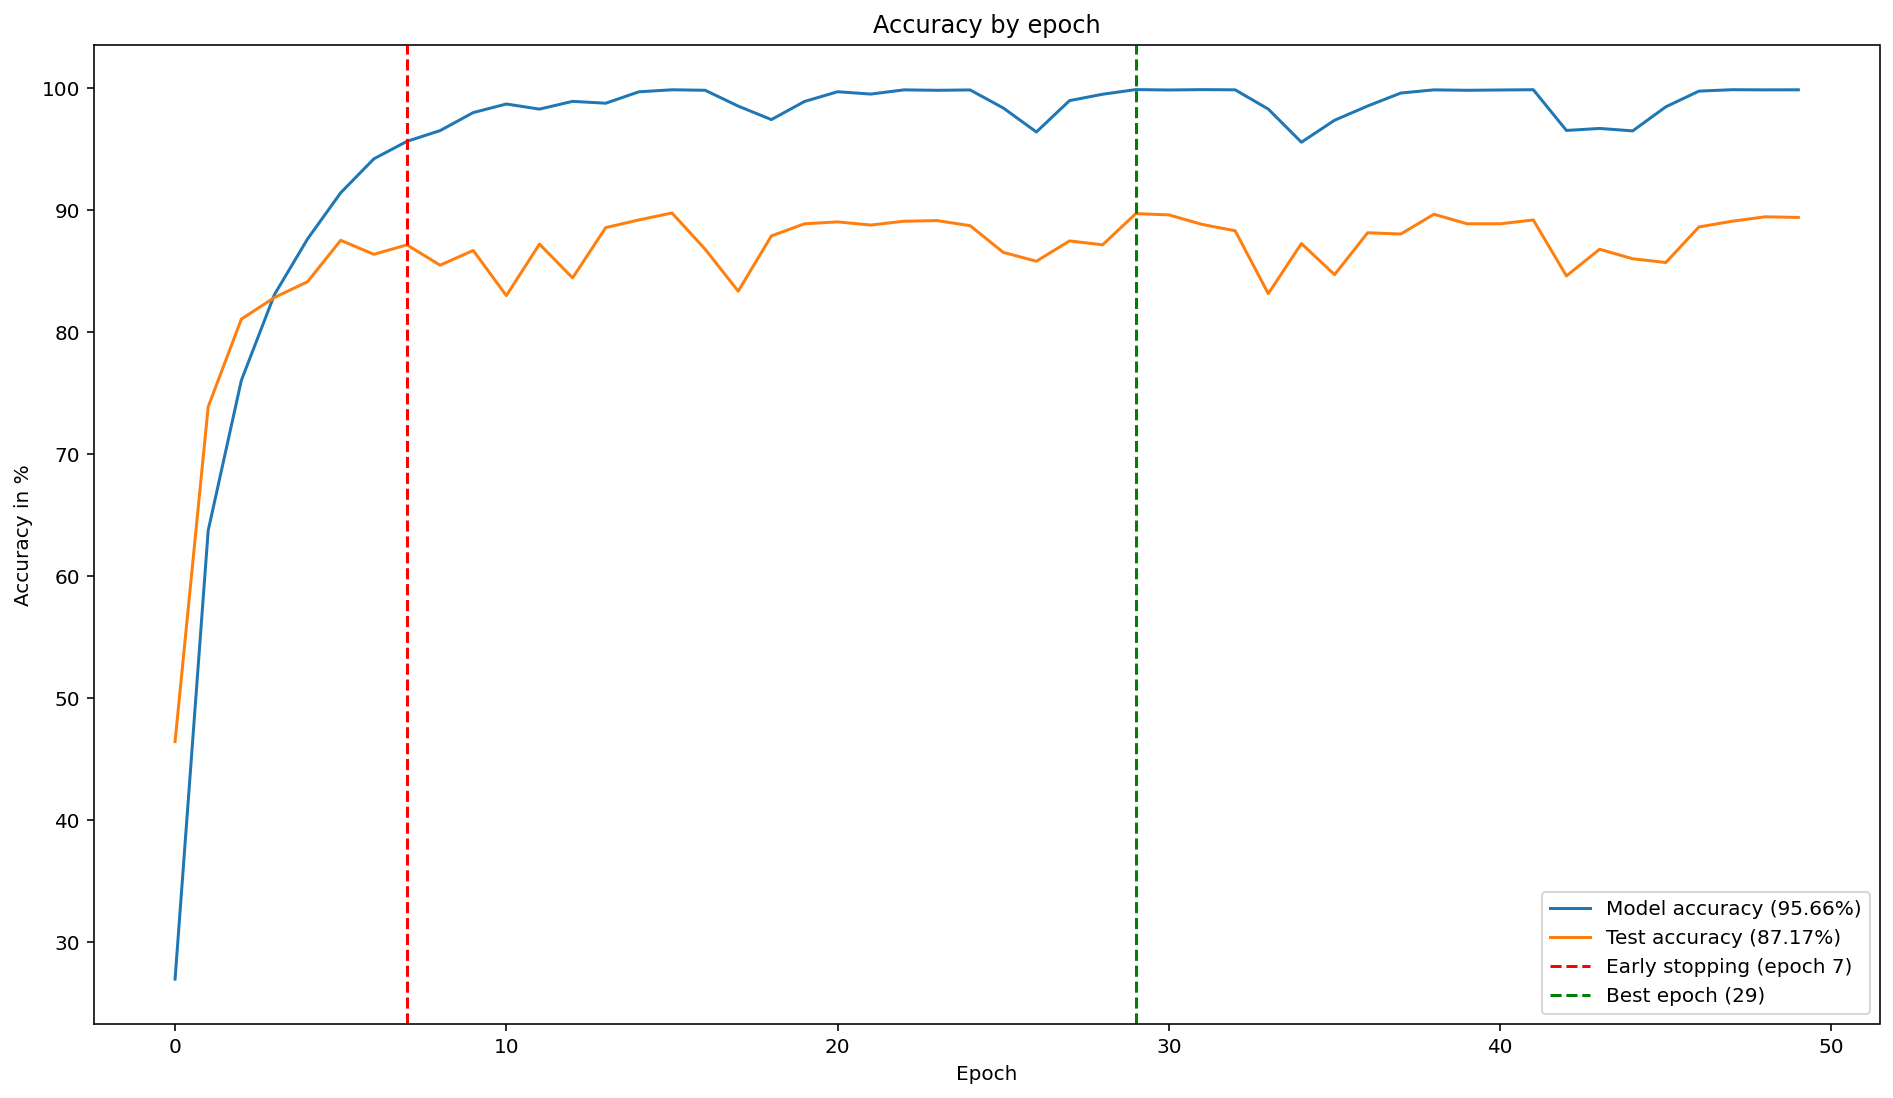
\includegraphics[width=1\textwidth]{assets/alexnet_accuracy.png}
    \caption{AlexNet accuracy by epoch.}
    \label{fig:alexnet_accuracy}
\end{figure}

\begin{figure}
    \centering
    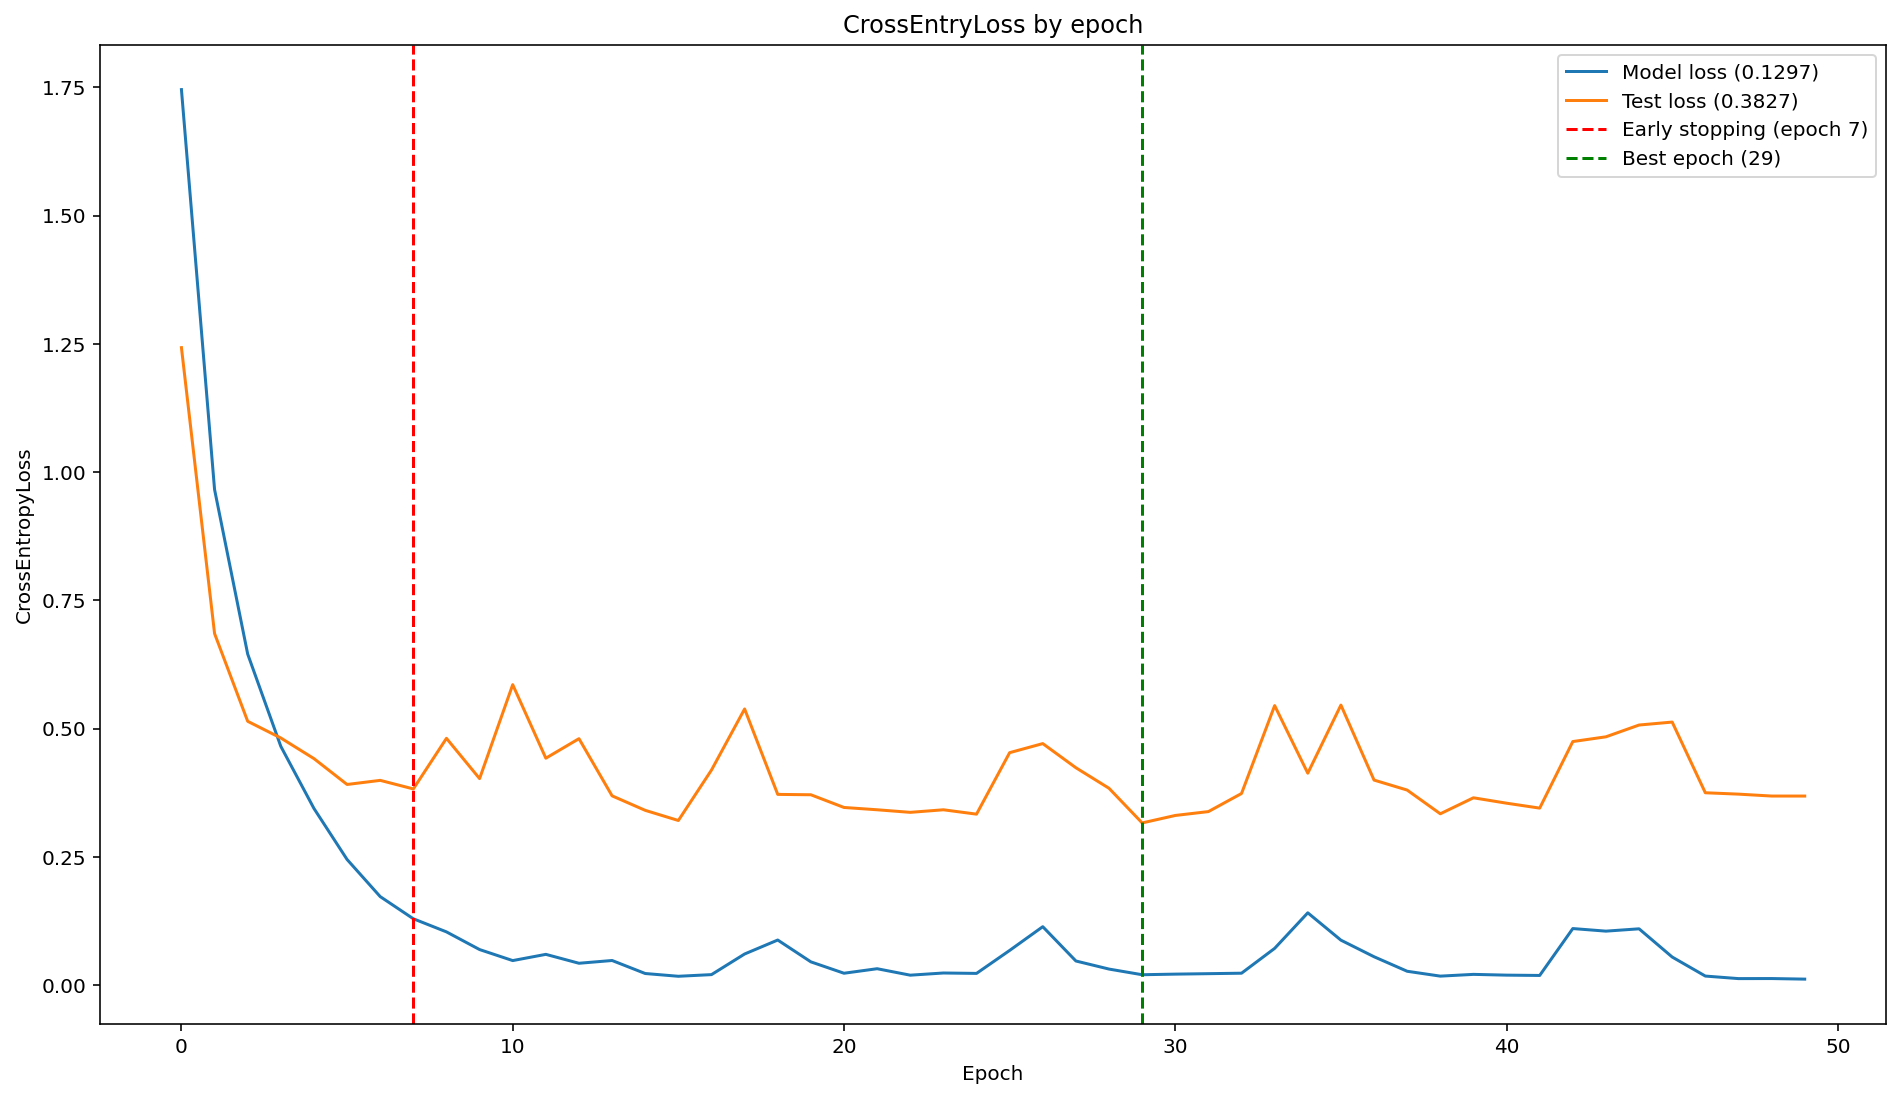
\includegraphics[width=1\textwidth]{assets/alexnet_loss.png}
    \caption{AlexNet cross-entropy loss by epoch.}
    \label{fig:alexnet_loss}
\end{figure}

\subsection*{ResNet18 Model}
\label{app:appendix_resnet_model}
\begin{figure}
    \centering
    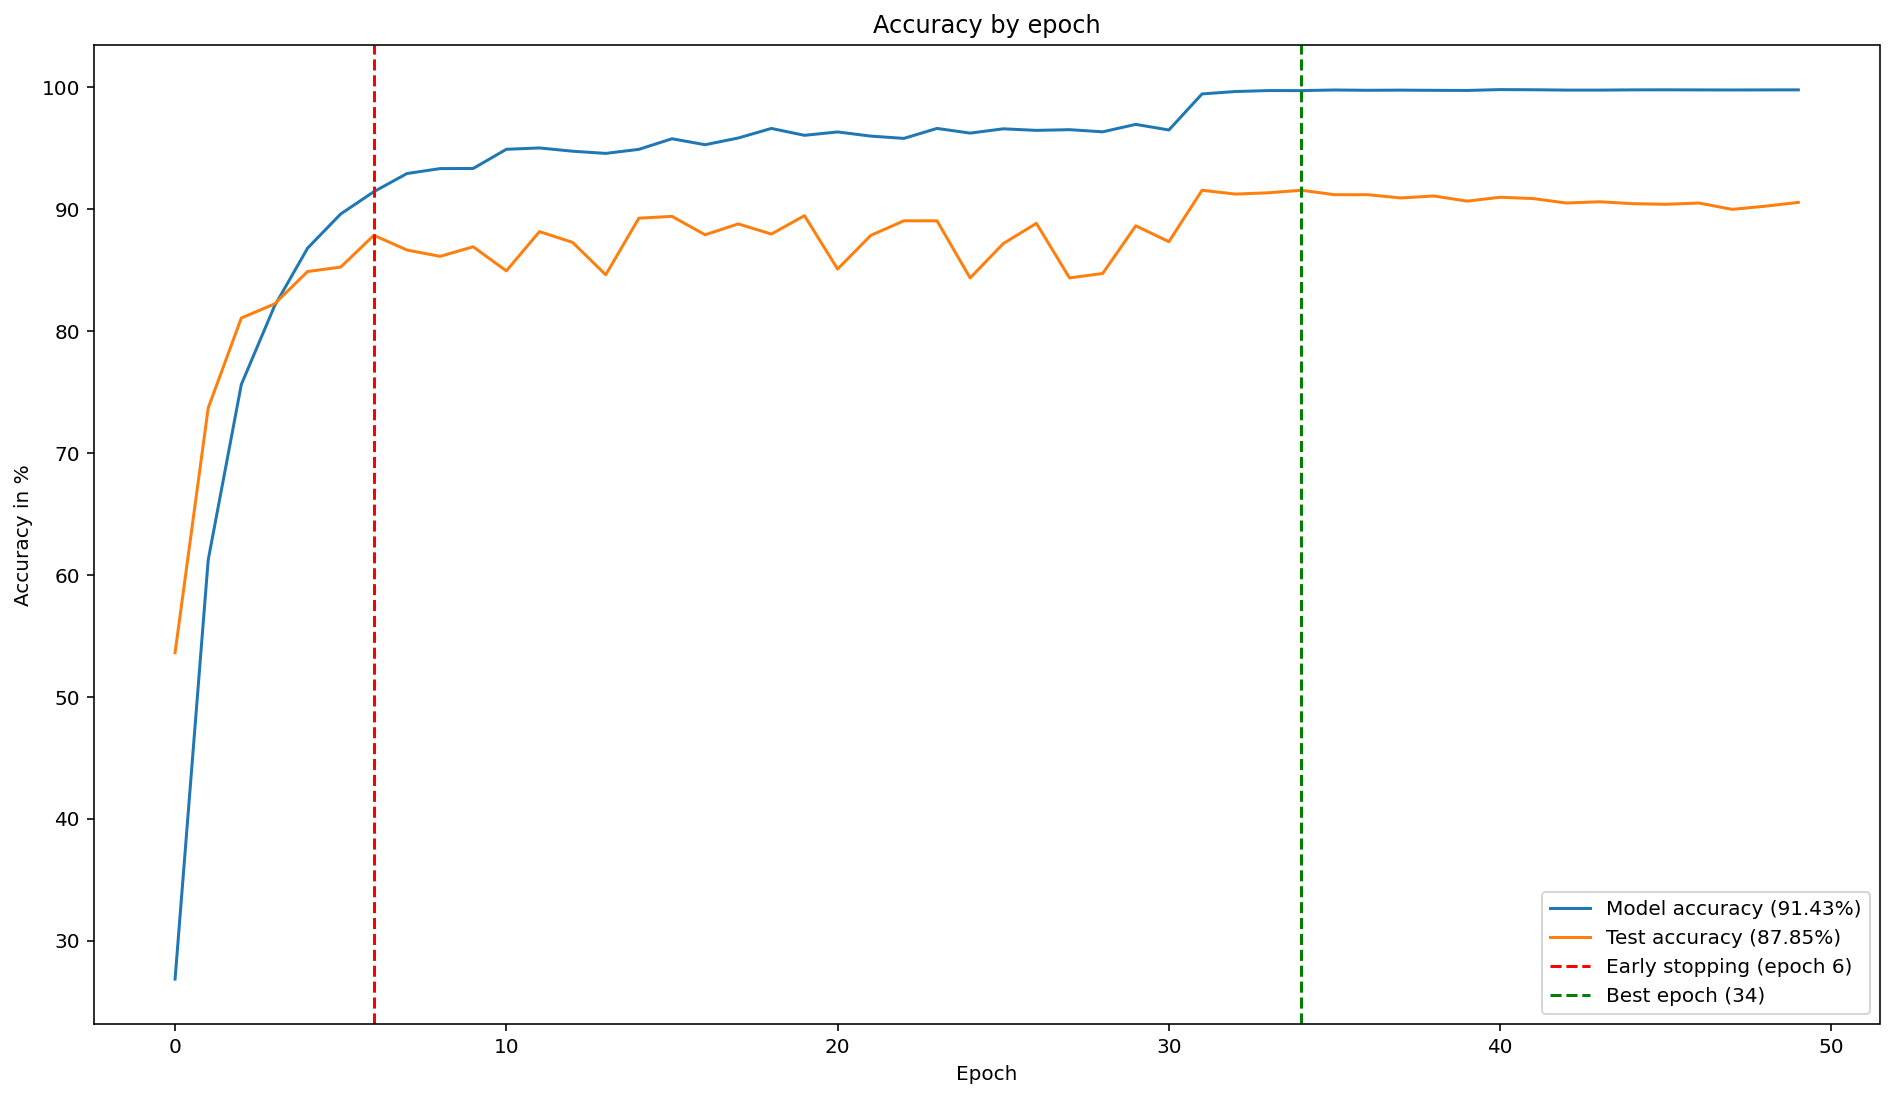
\includegraphics[width=1\textwidth]{assets/resnet_accuracy.png}
    \caption{ResNet18 accuracy by epoch.}
    \label{fig:resnet_accuracy}
\end{figure}
\begin{figure}
    \centering
    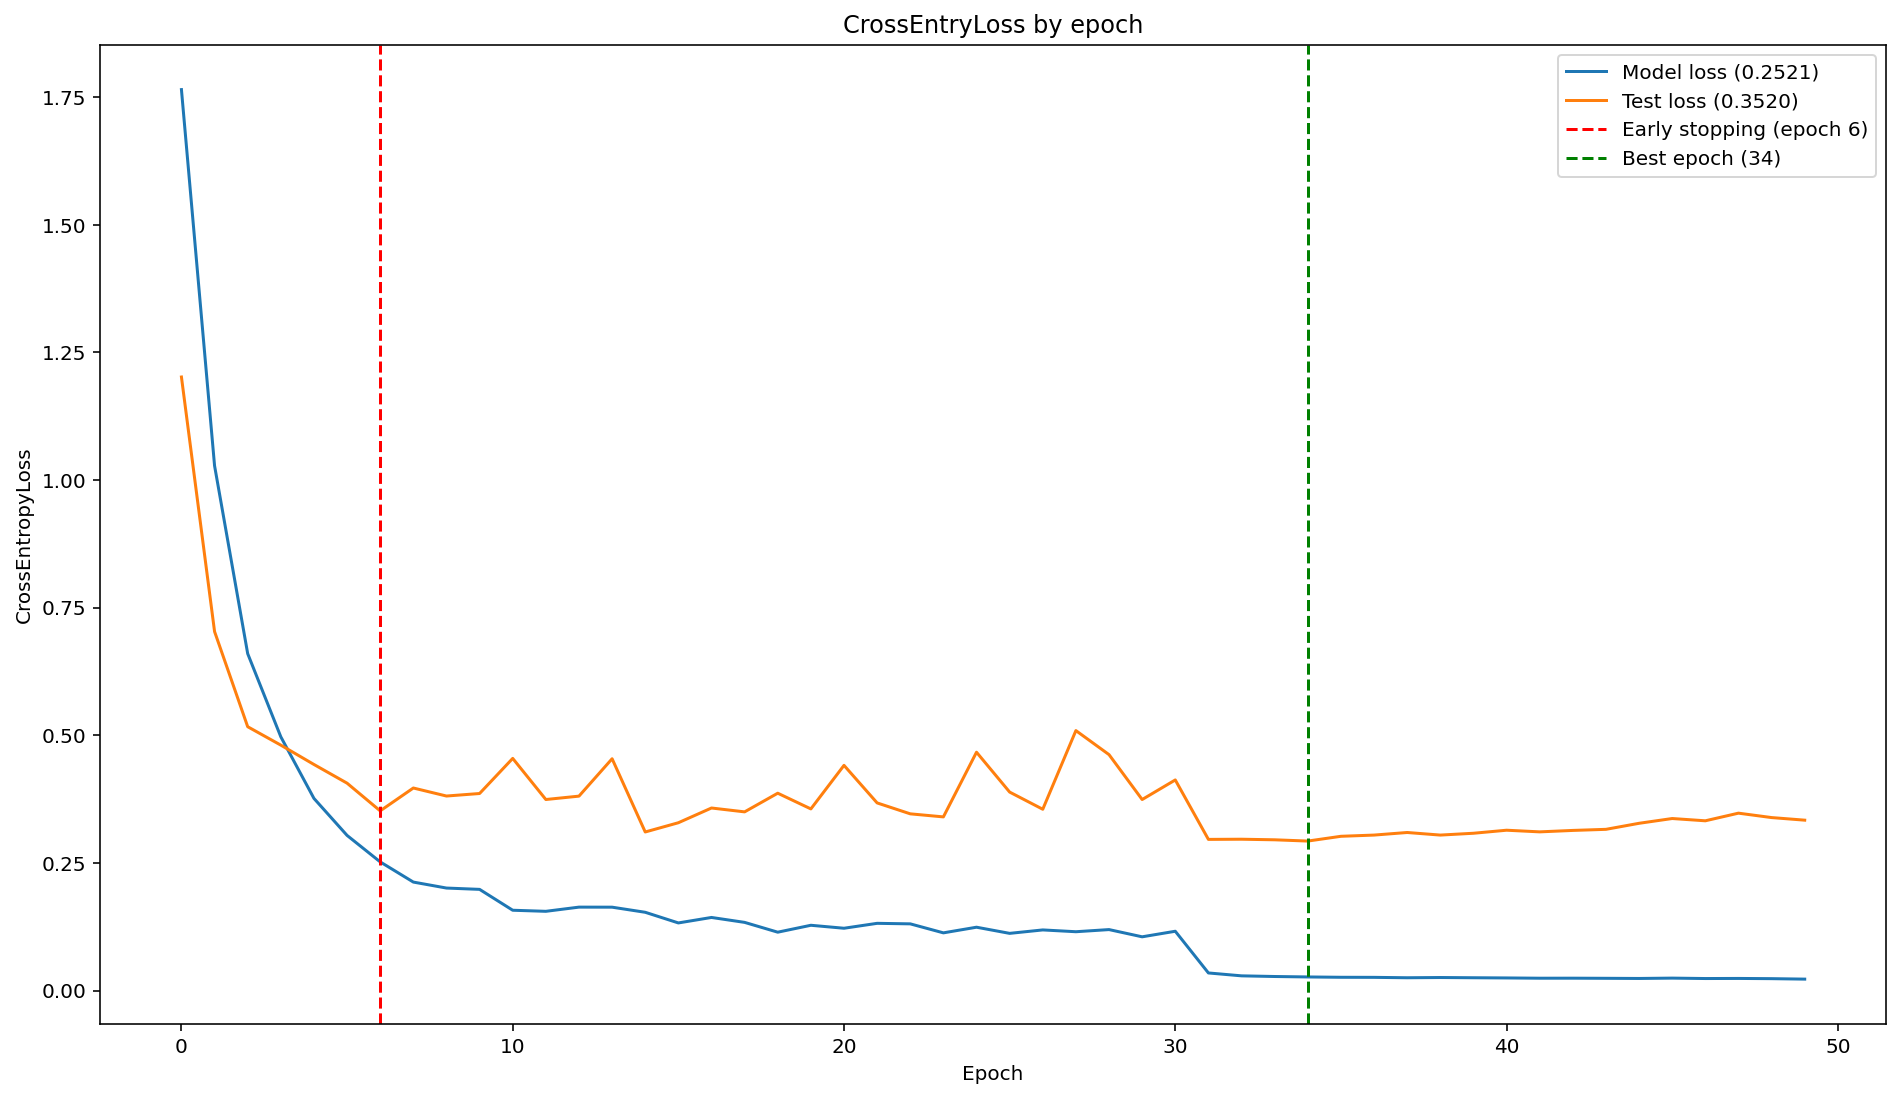
\includegraphics[width=1\textwidth]{assets/resnet_loss.png}
    \caption{ResNet18 cross-entropy loss by epoch.}
    \label{fig:resnet_loss}
\end{figure}

\subsection*{Relational Data Model}
\label{app:appendix_relational_data_model}
\begin{figure}[ht]
\label{fig:erd}
\centering
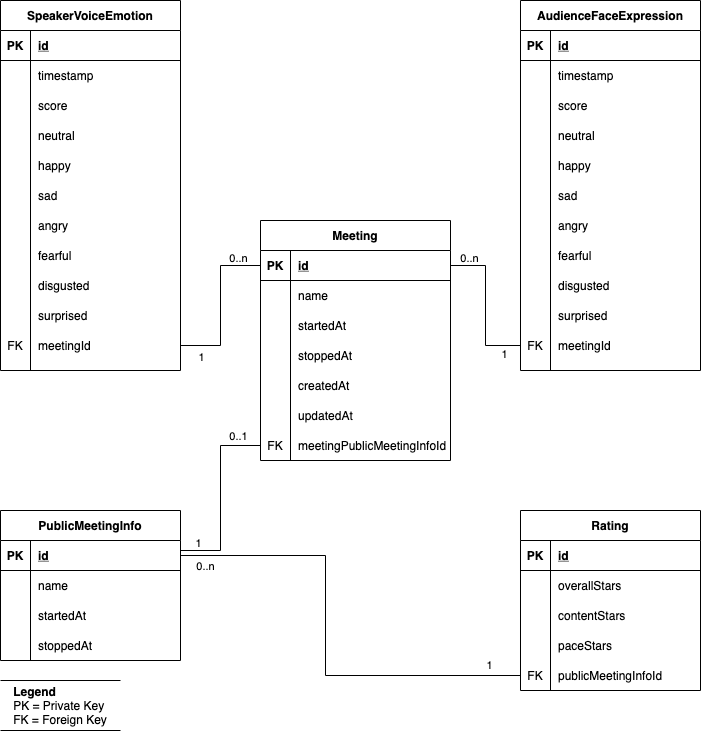
\includegraphics[width=1\textwidth]{assets/erd.png}
\caption{The entity relationship diagram (ERD) for the database structure of Moody. Relationships are modeled in UML style. Each table has an additional owner field  storing the user id from AWS Cognito which is omitted in the illustration for brevity.}
\end{figure}

\subsection*{Source Code}
\label{app:appendix_source_code}
All source code related to the Moody application can be found at the GitHub organization \texttt{COINS-SS21}: \url{https://github.com/COINS-SS21}.

\begin{itemize}
    \item Web application: \url{https://github.com/COINS-SS21/moody}
    \item Speech emotion recognition model: \url{https://github.com/COINS-SS21/moody-ser}
    \item \LaTeX{} source of this paper: \url{https://github.com/COINS-SS21/moody-paper}
\end{itemize}
